\subsection{Anomalous Magnetic Moment of the Muon}
The NP contributions for the anomalous magnetic moment of the muon are discribed by the parameter set 
\begin{align}
 \left(m, M_l, g_2^l\right).
\end{align}
The Feynman diagram for this process is depicted in figure \ref{pic_g-2}. 
\begin{figure}[t]
 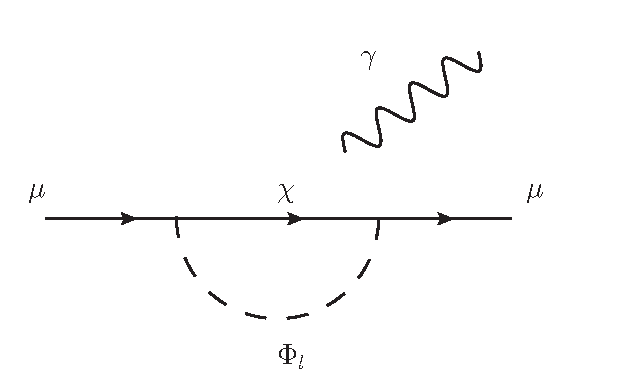
\includegraphics[width=0.6\textwidth]{../pics/g-2.eps}
 \caption{One-loop contribution to $a_\mu$. Depending on the representations, there are multiple possibilites to attach the photon.}
 \label{pic_g-2}
\end{figure}
Depending with which particle in the loop the photon interacts, there is a different matrix element. If it couples to the scalar, it reads
\begin{align}
 M^\rho = |g_2^l|^2 Q_B e \int \frac{\dx^4 k}{(2\pi)^4} \bar\mu_L(p_2) \frac{\slashed{k}+m_\chi}{D_F}\mu_L(p_1) \frac{1}{D^l_{k-p_1}}\left(2k-p_1-p_2\right)^\rho\frac{1}{D^l_{k-p_2}}
\end{align}
where $Q_B$ is the electric charge of the boson, $\ti e(q_1-q_2)^\mu$ is the scalar-photon coupling (MDSchwartz) and $D_F$ is the denominator of the
DM fermion. The free Lorentz-index gets contracted with
the polarisation vector $\epsilon_\rho$ of the external photon. As before, due to the chiral muons, only the $\slashed{k}$ in the internal fermion
propagator remains and leaves a $\gamma^\mu$ in between the muon fields. Thereof the operator $\sfrac{\sigma^{\mu\nu}q^\nu}{2m}$ can be inserted with the Gordon 
identity \eqref{eq_gordon} so that we are left with computing 
\begin{align}
 M^\rho_{(\mu)} \propto \int\frac{\dx^4 k}{(2\pi)^4} \left[ \frac{2k_\mu k^\rho}{D^\chi_kD^l_{k-p_1}D^l_{k-p_2}} - \frac{k_\mu}{D^\chi_kD^l_{k-p_1}D^l_{k-p_2}}\left(p_1 +p_2\right)^\rho \right].
\end{align}
Don't miss that the index $\mu$ is contracted with the Dirac-tensor $\sigma$ which is omitted here. With \cite{Lavoura} we get
\begin{align}
 \int\frac{ k^\rho k_\mu}{D^\chi_kD^l_{k-p_1}D^l_{k-p_2}} =&  f (p_1^\rho p_{2\mu} + p_2^\rho p_{1\mu}) +  d_1p_1^\rho p_{1\mu} +  d_2p_2^\rho p_{2\mu} + \bar x g^\rho_\mu\\
 \int\frac{k_\mu}{D^\chi_kD^l_{k-p_1}D^l_{k-p_2}} =&  c_1 p_{1\mu} +  c_2 p_{2\mu},
\end{align}
where $c_i$, $d_i$, $f$ are here not further specified loopfunctions $\sim \sfrac{1}{m^2_\chi} \cdot g(x_l)$, $g$ being a smooth function. The divergent $x$
cancels out with two-point functions. Note that their notation is slightly different to ours due to the relative inversion of the squared mass 
fraction $x_l$. In the massless limit $m_1^2 = m_2^2 = 0$ we obtain $d_1 = d_2 = 2f =: d$ and $c_1 = c_2 =: c$. Our matrix element now is
\begin{align}
 M^\rho_{(\mu)} \propto (p_1^\rho p_{2\mu} + p_2^\rho p_{1\mu}) (d-c) + (p_1^\rho p_{1\mu} + p_2^\rho p_{2\mu}) (2d-c).
\end{align}
We can use $q^2 = (p_1-p_2)^2 = 0$ for an on-shell photon and again $p^\rho p_\mu = \sfrac{1}{4} p^2 g^\rho_\mu $ which leaves our eventual form factor 
Lorentz-invariant. After gathering everything up and performing the calculation for the fermionic case, we have
\begin{align}
 M^\rho = \frac{|g^l_2|^2}{16\pi^2} \frac{m^2_\mu}{m_\chi^2}\left(Q_\chi^i I(x_l) + Q_{\Phi_l}^i \frac{1}{x_l} I(x_l^{-1}) \right)\times \bar \mu_L\frac{e\ti\sigma^{\rho\nu}q_\nu}{2m_\mu} \mu_L,
 \label{eq_g-2}
\end{align}
where the sum over $i$ is understood so that for the electric charges, $Q_\mu = Q_\chi - Q_{\Phi_l}$ is ensured and
\begin{align}
 I(x) = \frac{1}{12(x-1)^4}\left(2+3x-6x^2+x^3+6x\log(x) \right) \stackrel{x\rightarrow1}{=} \frac{1}{24}.
\end{align}
The NP contribution to $\Delta a_\mu$ can be read off \eqref{eq_g-2}.
